\documentclass[12pt]{book}







\usepackage[a4paper, margin=3cm]{geometry}
\usepackage[english]{babel}
\usepackage[utf8]{inputenc}
% \usepackage{bookman}
\usepackage{amsmath}
\usepackage{amssymb}
\usepackage{amsthm}
\usepackage{syntax}
\usepackage{tikz}
\usepackage{xcolor}
\usepackage{forest}
\usepackage{mathtools}
\usepackage{tikz-cd}
\usepackage{mathrsfs}
\usepackage{stmaryrd}
\usepackage{enumitem}
\usepackage{listings}
\usepackage{xcolor}
\usepackage{stmaryrd}
\usepackage{bussproofs}
\usepackage{amsmath,amssymb}
\usepackage{mathtools}
\usepackage{stmaryrd}
\usepackage{mathpartir}
\usepackage{tikz}
\usepackage{algorithm}
\usepackage{algpseudocode}
%\usepackage{minted}
%\usemintedstyle{bw}
\usetikzlibrary{positioning, arrows.meta}
\definecolor{refcolor}{RGB}{0, 0, 0}
\usepackage[
  colorlinks=true,
  linkcolor=refcolor,
  citecolor=refcolor,
  urlcolor=refcolor,
  pdfborder={0 0 0}
]{hyperref}
\usepackage{xcolor}
\usepackage{etoolbox}
\definecolor{keywordcolor}{rgb}{0.0,0.2,0.6}
\definecolor{commentcolor}{rgb}{0.3,0.5,0.3}
\definecolor{stringcolor}{rgb}{0.5,0.1,0.1}
\definecolor{bgcolor}{rgb}{0.95,0.95,0.95}
\lstdefinelanguage{Haskell}{
  morekeywords={
    case,class,data,default,deriving,do,else,if,import,in,infix,infixl,
    infixr,instance,let,module,newtype,of,then,type,where,forall
  },
  sensitive=true,
  morecomment=[l]--,
  morecomment=[n]{\{-}{-\}},
  morestring=[b]",
}

\lstdefinestyle{haskellstyle}{
  language=Haskell,
  basicstyle=\ttfamily\small,
  keywordstyle=\color{keywordcolor}\bfseries,
  commentstyle=\color{commentcolor}\itshape,
  stringstyle=\color{stringcolor},
  backgroundcolor=\color{bgcolor},
  showstringspaces=false,
  numbers=left,
  numberstyle=\tiny,
  numbersep=5pt,
  frame=single,
  breaklines=true,
  captionpos=b
}

\definecolor{leankeyword}{RGB}{0,0,180}
\definecolor{leancomment}{RGB}{0,128,0}
\definecolor{leanstring}{RGB}{163,21,21}

\lstdefinelanguage{Lean4}{
  morekeywords={
    def, inductive, structure, theorem, variable, variables,
    namespace, end, match, with, open, import, let, in, if, then, else,
    Type, Prop, fun, forall, do, where, deriving, instance
  },
  sensitive=true,
  morecomment=[l]--,
  morestring=[b]",
  morestring=[b]`,
  keywordstyle=\color{leankeyword}\bfseries,
  commentstyle=\color{leancomment}\itshape,
  stringstyle=\color{leanstring},
  basicstyle=\ttfamily\small,
  columns=fullflexible,
  keepspaces=true,
  showstringspaces=false
}

\newcommand{\la}{\lambda}
\newcommand{\La}{\mathbf{\Lambda}}
\newcommand{\Vset}{\mathbf{V}}
\newcommand{\NAT}{\mathbb{N}}
\newcommand{\IF}{\texttt{IF}}
\newcommand{\SUCC}{\texttt{SUCC}}
\newcommand{\TRUE}{\texttt{TRUE}}
\newcommand{\FALSE}{\texttt{FALSE}}
\newcommand{\FST}{\texttt{FST}}
\newcommand{\SND}{\texttt{SND}}
\newcommand{\PAIR}{\texttt{PAIR}}
\newcommand{\NIL}{\texttt{NIL}}
\newcommand{\NOT}{\texttt{NOT}}
\newcommand{\AND}{\texttt{AND}}
\newcommand{\OR}{\texttt{OR}}
\newcommand{\cat}[1]{\mathbf{#1}}
\newcommand{\Hom}{\mathrm{Hom}}
\newcommand{\id}{\mathrm{id}}
\newcommand{\Ob}{\mathrm{Ob}}
\newcommand{\Mor}{\mathrm{Mor}}
\newcommand{\Set}{\cat{Set}}
\newcommand{\Top}{\cat{Top}}
\newcommand{\Grp}{\cat{Grp}}
\newcommand{\Fun}{\mathrm{Fun}}
\newcommand{\op}{^{\mathrm{op}}}
\newcommand{\lCalc}{$\la$-Calculus}
\newcommand{\lcalc}{$\la$-calculus}
\newcommand{\bred}{$\beta$-reduction}
\newcommand{\lterm}{$\la$-term}
\newcommand{\lterms}{$\la$-terms}
\newcommand{\lexpr}{$\la$-expression}
\newcommand{\aequiv}{$\alpha$-equivalence}
\newcommand{\aequivlt}{$\alpha$-equivalent}
\newcommand{\bequiv}{$\beta$-equivalence}
\newcommand{\functionfont}[1]{\mathbf{#1}}
\newcommand{\curly}{\mathrel{\leadsto}_\beta}
\newcommand{\Sub}[1]{\functionfont{Sub}(#1)}
\newcommand{\Subb}{\functionfont{Sub}}
\newcommand{\FV}[1]{\functionfont{FV}(#1)}
\newcommand{\FVV}{\functionfont{FV}}
\newcommand{\orange}[1]{\textcolor{orange}{#1}}
\newcommand{\magenta}[1]{\textcolor{magenta}{#1}}
\newcommand{\blue}[1]{\textcolor{blue}{#1}}
\newcommand{\green}[1]{\textcolor{green}{#1}}
\newcommand{\myref}[1]{\textcolor{refcolor}{\hyperref[#1]{\ref*{#1}}}}
\newcommand{\subst}[2]{[#1 := #2]}
\newcommand{\step}{\curly}
\newcommand{\etaequiv}{$\eta$-equivalence}
\newcommand{\lam}[2]{\lambda #1.\,#2}
\newcommand{\app}[2]{#1.\,#2}
\newcommand{\abs}[2]{\la #1.\,#2}
\newcommand{\curlysym}{\mathrel{\leftrightarrow}_\beta}
\renewcommand{\arraystretch}{1.2}
\setlength{\tabcolsep}{12pt}

\theoremstyle{definition}
\newtheorem{theorem}{Theorem}[section]
\newtheorem{lemma}[theorem]{Lemma}
\newtheorem{corollary}[theorem]{Corollary}
\newtheorem{definition}{Definition}[section]
\newtheorem{example}{Example}[section]
\newtheorem{remark}{Remark}
\newtheorem{proposition}[theorem]{Proposition}
\newtheorem{note}{Note}

\bibliographystyle{alpha}

\title{Type Theory and Categorical Models: A Unified Approach}
\author{Miguel Laredo}





\begin{document}

\chapter{\lCalc}

In the early 20th century, mathematicians such as Bertrand Russell, David Hilbert, and Kurt Gödel were trying to set complete, consistent, and decidable foundations for mathematics. Within this context, Alonzo Church, in his effort to formalize the notion of  computability, introduced a minimal symbolic language based upon function abstraction and function application, this system is now called \lcalc.

In 1936, Church used lambda calculus to address Hilbert’s Entscheidungsproblem --whether a mechanical method could determine the truth of any first-order logic statement. He proved no such algorithm exists, establishing the undecidability of first-order logic.

One of the nuances formalized by the \lcalc \ is the distinction between extensional and intensional equality. The extensional approach to equivalence states that two functions are equivalent if they share input output pairs for every possible input. Its intensional counterpart extends this notion of equality by requiring that the procedures that compute these pairs share complexity i.e. they take the same steps toward yielding a result.\footnote{
  Let \( p \) be a sufficiently large prime, and let \( f, g : \mathbb{Z}_p \to \mathbb{Z}_p \) be defined by \( f(x) = x^2 \) and \( g(x) = \log_a(a^{x+2}) \), where \( a \in \mathbb{Z}_p^\times \) is a fixed primitive root. Although \( f \) and \( g \) are extensionally equal, i.e., they yield the same output for all inputs in \( \mathbb{Z}_p \), they are intensionally distinct. The function \( f \) performs a simple squaring operation, while \( g \) requires evaluating a discrete logarithm, intractable in general. \magenta{[Pedro Bonilla]}
}

Languages like LISP, Haskell, Erlang and others share the \lcalc \ as their theoretical foundation. The lambda calculus has established itself as the backbone of functional programming. The introduction of type systems into the \lcalc \ has allowed us to computer-verify mathematical proofs and develop programs that are correct by construction.\footnote{Principles of the \lcalc \ and Type Theory underlie every computer assisted verification tool as well as proof assistants and kitchen table programming languages like C or Java.}


\newpage
\section{\centering Untyped \lCalc}
In order to get acquainted with the \lcalc, let us develop a simple example to familiarize ourselves before we begin with a more formal approach to this discipline. Consider the function $f(x) = x + 1$, the most straightforward way to express this using \lcalc \ would be $(\la x . x + 1 )$, where the lambda denotes that $x$ is being captured and used as a parameter to perform some computation\footnote{this is an e.g., $(\la x . x + 1 )$ is not a valid lambda term, see Definition \ref{def:lambda-terms-2}.}. Evaluating $f(2)$ using this newly created lambda term would look like this: $(\la x . x + 1)(2) \curly (2 + 1) \curly 3$. This process of reducing a $\la$-expression is referred to as \bred, it will be covered formally later in the chapter.

\begin{definition} The set of all lambda terms \( \La \) is defined inductively as follows:
  \label{def:lambda-terms-1}
  \begin{itemize}
  \item (Variable) If \( x \in \Vset \), then \( x \in \La \).  
  \item (Abstraction) If \( x \in \Vset \) and \( M \in \La \), then \( (\la x. M) \in \La \).
  \item (Application) If \( M, N \in \La \), then \((M N) \in \La \).
  \end{itemize}
  Where $\Vset = \{x, y, z, ... \}$ represents a countably infinite set of variable names.
\end{definition}
  
The key takeaway of this definition is that abstraction and application together, when combined with \bred, enable computation—thus encapsulating the meaning of function in a way that is abstract yet useful.

Since we are dealing with a formal language, it is in our benefit to introduce a few other objects with the aim of defining a grammar to generate the set $\La$:
\begin{itemize}
\item An alphabet \( \Sigma = \{ \la, ., (, ), \ldots \} \), is a finite set of symbols
\item A string is a finite sequence of elements from \( \Sigma \), the empty string is denoted by \( \varepsilon \)
\item \( \Sigma^* \) denotes the set of all finite strings over \( \Sigma \), \( \varepsilon \in \Sigma^* \)
\item A language \( L \) over an alphabet \( \Sigma \) is a subset of \( \Sigma^* \)
\end{itemize}
Our aim now, to generate the set $\La$,  to do this, we will make use of a grammar. When dealing with grammars that define programming languages i.e. context-free grammars, Backus-Naur Form, BNF for short is the way to go:
\begin{itemize}
\item Nonterminals are enclosed in angle brackets (e.g. \texttt{<expr>})
\item Terminals are written literally (e.g. \texttt{"$\lambda$"}, \texttt{"."}, $x$)
\item Productions define how nonterminals expand, written as \texttt{::=}
\item The vertical bar \texttt{|} denotes available expansions
\end{itemize}
Thus, the language for natural numbers in decimal notation is represented using:
\begin{align*}
  \texttt{<digit>} &\;\texttt{::=}\; \texttt{"0"} \;\texttt{|}\; \texttt{"1"} \;\texttt{|}\; \texttt{"2"} \;\texttt{|}\; \texttt{"3"} \;\texttt{|}\; \texttt{"4"} \;\texttt{|}\; \texttt{"5"} \;\texttt{|}\; \texttt{"6"} \;\texttt{|}\; \texttt{"7"} \;\texttt{|}\; \texttt{"8"} \;\texttt{|}\; \texttt{"9"} \\
  \texttt{<number>} &\;\texttt{::=}\; \texttt{<digit>} \;|\; \texttt{<digit>} \ \texttt{<number>}
\end{align*}
\begin{definition} Taking advantage of BNF notation, an alternative definition for $\La$ would be:
  \label{def:lambda-terms-2}
  \begin{align*}
    \texttt{<term>} &\;\texttt{::=}\; \texttt{<variable>} \\
                    &\;\texttt{|}\; \texttt{"$\la$"}\ \texttt{<variable>}\ \texttt{"."}\ \texttt{<term>} \\
                    &\;\texttt{|}\; \texttt{"("}\ \texttt{<term>}\ \texttt{<term>}\ \texttt{")"} \\
    \texttt{<variable>} &\;\texttt{::}\in \Vset
  \end{align*}
  where \( \Sigma = \{ \la, ., (, )\} \cup \Vset \) and \( \La \subset \Sigma^* \). Through use of inductive types types\footnote{Inductive Data Types are inductively defined types built from sums (either this or that) of products (this and that). They let you define structured data with multiple forms and support safe, exhaustive pattern matching. }, this grammar can be implemented in Lean4:

\end{definition}
\begin{remark}
  From the definition above we extract that \( \lambda x . x + 1 \notin \La \), given this circumstance, the need to find an accurate representation for numbers within this definition arises. See Definition \ref{def:church-naturals}
\end{remark}
\begin{example} \label{ex:lambda-terms} Some examples of valid $\la$ terms generated using the grammar in \ref{def:lambda-terms-2}:
  \( y \),
  \( (\la x. (x x)) \),
  \( (\la x. (\la y. x)) \),
  \( (((\la x. (x y)) (\la y. y)) z) \).
  The Lean4 counterpart for the second term is:
\end{example}
As a convention to avoid notational cluttering, the outermost parenthesis can be omitted e.g. $ ( \la x.x ) $ can be read as $ \la x.x $. Also, application is left-associative  and binds tighter than abstraction, so $M N P$ is parsed as $(M N) P$ and $\la x . M N$ means $\la x . (M N)$, not $(\la x . M) N$. Likewise, abstraction is right-associative e.g. $\la x . \la y . M$ is $\la x . (\la y . M)$ and binds more weakly than application. All these are just to keep notation straight-forward, the formal definition does not leave precedence under-specified thanks to parenthesis. Those interested in the implementation need not worry, as Lean4 enforces an explicit order on constructors.
\subsection{\centering Equivalence of terms}
Having defined the language of the \lcalc, we move on to the mechanics of computation. To this end, several equivalences among terms will be defined, namely \aequiv, \bequiv, and \etaequiv
. Every lambda term is made up of other smaller lambda terms, so it is only natural to define the set that contains all subterms of a given term:
\begin{definition} Given $T \in \La$, $\functionfont{Sub} : \La \to \mathcal{P}(\Vset)$ maps a term to the set of it's subterms.
  \begin{align*}
    &\Sub x = \{x\} \\
    &\Sub {MN} = \Sub M  \cup \Sub N \cup \{MN\} \\
    &\Sub {\la x . M} = \Sub M  \cup \{\la x. M\}
  \end{align*}
  Where $x \in \Vset$ and $M, N \in \La $.

\end{definition}
\begin{remark}
  Let \( \preceq \) be the subterm relation on \lterms, defined by
  \[
    M \preceq N \iff M \in \Sub{ N }
  \]
  \( \preceq \) is a partial order relation. This statement is follows intuitively from the definition, it can be proven using induction on the derivation tree.
\end{remark}
\begin{definition} A term $ S \in \Sub M, \ M \in \La$ is said to be proper if $S \neq M$. $\Sub{M} \setminus \{M\}$ would be the set of proper subterms.
\end{definition}
\begin{definition} Let \( M = \lambda x. N \) be a \lterm:
  \begin{itemize}
  \item The variable \( x \) is the binding variable of the abstraction \( \lambda x. N \).
  \item An occurrence of a variable \( x \) in \( M \) is bound if \( x \in \Sub { \lambda x. N } \).
  \item Free variables are those that are not bound.
  \end{itemize}
\end{definition}
\begin{example}
  Take $ M \equiv \la x . \, x \, y $, in this example, the $x$ in $\la x. $ is binding, $y$ is free, and $x$ is bound. This means that $y$ is used literally, and that $x$, as denoted by $\la x.$ is abstracted and thus subject to being replaced within the context of said abtraction. A subexample might make this explicit: $ (\la x . \, x \, y) \, M \curly M \, y $. The $y$ remained while the $x$ was used as a placeholder for $M$.
\end{example}
\begin{remark}
  This taxonomy is key to understanding concepts such as \aequiv \ intuitively.
\end{remark}
The set of Free Variables $\functionfont{FV}$, those that will not get replaced during the process of reduction, is computed using:
\begin{definition} Given $T \in \La $, $\functionfont{FV} : \La \to \mathcal{P}(\Vset) $ outputs the set of free variables for $T$:
  \begin{align*}
    & \FV x = \{x\}\\
    & \FV {MN} = \FV M \cup \FV N \\
    & \FV {\lambda x . M} = \FV M \setminus \{x\}
  \end{align*}
  Where $ x \in \Vset $ and $ M, N \in \La $, and $\mathcal{P}$ denotes the power set.

\end{definition}
\begin{example} Computing the free variables of $\lambda x . \lambda y . y x z$. The term well-formed, so we proceed:
  \begin{align*}
    \FV {\lambda x . \lambda y . y x z} &= \FV {\lambda y . yxz} \setminus \{x\} \\
                                        &= \FV {yxz} \setminus \{x, y\} \\
                                        &= \{x, y, z\} \setminus \{x, y\} \\
                                        &= \{z\}
  \end{align*}
  Of course, $z$ is the only free variable in the expression as it is the only variable that is not captured by some $\la$-abstraction.
\end{example}
\begin{definition}
  A term $M \in \La$ is closed if and only if $\FV M = \emptyset$, closed lambda terms are often referred to as combinators. $\La^0$ is the set of all closed lambda terms.
\end{definition}
\begin{note} They are called combinators since having no free variables means that all variables are bound, and thus, a closed term just combines bound variables.
\end{note}

We aproach the definition for \aequiv \, to this end we have to introduce what it means to substitute a variable.

\begin{definition}Capture-Avoiding Substitution Rules
  Let \( M, N \in \La \) and \( x, y, z \in \Vset \). The substitution \( M[x := N] \) is defined inductively as:
  \[
    \begin{aligned}
      x[x := N]                       & = N \\
      y[x := N]                       & = y && y \neq x \\
      (M_1\, M_2)[x := N]             & = (M_1[x := N])\,(M_2[x := N]) \\
      (\lambda x. M)[x := N]          & = \lambda x. M \\
      (\lambda y. M)[x := N]          & = \lambda y. (M[x := N]) && y \neq x, y \notin \FV { N } \\
      (\lambda y. M)[x := N]          & = \lambda z. (M[y := z][x := N]) && y \neq x, y \in \FV { N }
    \end{aligned}
  \]
  where \( z \notin \FV { M } \cup \FV { N } \).
\end{definition}
Hopefully the meaning of the first three rules is clear, they ancapsulate renaming in the context of variables and applications. The subsequent rules are about abstractions, rule four states that renaming a binding variable has no effect, renaming only modifies a term whenever the renamed variable is different from the binding variable. Rule five is the general case, that is, when the substitution just moves in together with the abstracted term. Then there is the last case, when the binding variable is a bound occurrence in the term we are substituting, which poses a problem, to see why, let us work through an example:
\begin{example} If by mistake we substitute $x$ by \( (\la w . \, w \, y) \) in \( (\la y . \, y \, x ) \) using rule five, we get:
  \[
    (\la y . \, y x) [x := (\la w . \, w \, y)] = (\la y . \, y \, (\la w. \, w \, y))
  \]
  We run into a problem. See that the free variable $y$ became bound after the rename. Free and bound variables should mantain their freedom or their boundedness after the rename, hence the need for rule 6, where we rename the binding variable to avoid the name clash:
  \[
    (\la y . \, y x) [x := (\la w . \, w \, y)] = (\la z . \, z \, (\la w. \, w \, y))
  \]
  
\end{example}
\begin{definition} Two lambda terms \( M, N \in \La \) are \aequivlt, written \( M =_\alpha N \), if they are structurally identical except for the names of bound variables.
  Formally:
  \[
    \begin{array}{@{}l@{\quad}l@{}}
      \inferrule*[right=\textsc{Alpha}]
      { }
      { \lam{x}{L} =_\alpha \la y . \, L \subst{x}{y} }
      &
        \inferrule*[right=\textsc{Abs}]
        { L =_\alpha L' }
        { \lam{x}{L} =_\alpha \lam{x}{L'} } \\[2ex]
      \inferrule*[right=\textsc{AppL}]
      { L_1 =_\alpha L_1' }
      { L_1\,L_2 =_\alpha L_1'\,L_2 }
      &
        \inferrule*[right=\textsc{AppR}]
        { L_2 =_\alpha L_2' }
        { L_1\,L_2 =_\alpha L_1\,L_2' }
    \end{array}
  \]
  $\alpha$-equivalence is an equivalence relation:
  \[
    \begin{aligned}
      &(Reflexivity) \quad && M =_\alpha M \\
      &(Symetry) \quad && M =_\alpha N \Rightarrow N =_\alpha M \\ 
      &(Transitivity) \quad && M =_\alpha N \text{ and } N =_\alpha P \Rightarrow M =_\alpha P
    \end{aligned}
  \]
\end{definition}
\begin{example} A simple equivalence class and two samples of not $\alpha$-equivalent \ pairs.
  \[
    \la x.\la y. \, y =_\alpha \la a.\la b. \, b =_\alpha \la z.\la x. \, x
  \]
  \[
    \la x. \la y. \, x \not=_\alpha \la x. \la y. \, y \quad \la x. \, x \, y \not=_\alpha \la x. \, x \, z 
  \]
  Remember terms are $\alpha$-equivalent \ only when bounded names are properly substituted.
\end{example}
\begin{remark}
  \aequiv \ comes naturally once substitution is defined, since the names of bound variables are just placeholders whose only purpuse is to get replaced.
\end{remark}
Naming variables can be a nightmare, which is why there exists a way of methodically assigning numbers to variables in a way that eliminates the need for \aequiv. These naming system works by using numeric indices that indicate how many binders away a variable’s binder is. These indices are called De Bruijn indeces.
\[
  \la x.\, x \Rightarrow \la.\, 0 \quad \la x. \la y.\, x \Rightarrow \la. \la.\, 1 \quad \la x. \la y.\, y \Rightarrow \la. \la. \, 0\,
\]
It turns out we are better at naming variables than at working with numbers, which is why we will stick to symbols and leave De Bruijn indices to computers. Programs like automated theorem provers do use this naming strategy to simplify their work.

\begin{definition} Single-step $\beta$-reduction $\step$ is defined using the following inference rules:
\[
\begin{array}{@{}l@{\quad}l@{}}
  \inferrule*[right=\textsc{Beta}]
    { }
    { (\lam{x}{M})\,N \step M\subst{x}{N} }
  &
  \inferrule*[right=\textsc{Abs}]
    { M \step M' }
    { \lam{x}{M} \step \lam{x}{M'} } \\[2ex]
  \inferrule*[right=\textsc{AppL}]
    { M_1 \step M_1' }
    { M_1\,M_2 \step M_1'\,M_2 }
  &
  \inferrule*[right=\textsc{AppR}]
    { M_2 \step M_2' }
    { M_1\,M_2 \step M_1\,M_2' }
\end{array}
\]
where \( M, N \in \La \). For those not familiar with inference rules, here is an alternative definition where \( L \in \La \)
\begin{itemize}
\item \( (\lam{x}{M})\,N \step M\subst{x}{N} \)
\item If $M \step N$, then: \( M\,L \step N\,L; L\,M \step L\,N; \lam{x}{M} \step \lam{x}{N} \)
\end{itemize}
\end{definition} 
Single \bred s can be applied succesively, which induces the following definition
\begin{definition} Zero or more step \bred, also called reflexive transitive closure. We write $M \step^* N$ if and only if there exists a sequence of one-step $\beta$-reductions starting from $M$ and ending at $N$.\footnote{The convention in the literature is to use $\rightarrow_\beta$ for \bred s $\twoheadrightarrow_\beta$ for multi-step \bred s. I prefer to use $\curly$ and $\curly^n$ since this allows me to use the superscript to note the number of steps in the process \bred \ e.g. $ (\la f. \la x . \, x) \, M \, N \curly^2 $ N. Instead of $\curly^n$ I use $\curly^*$ whenever the number of steps is undefined.}
  \label{def:zero-more-bred}
  \[
    M \equiv M_0 \step M_1 \step M_2 \step \cdots \step M_{n-1} \step M_n \equiv N
  \]
  That is, there exists an integer $n \geq 0$ and a sequence of terms $M_0, M_1, \dots, M_n$ such that: $ M_0 \equiv M $ and $ M_n \equiv N $ for all $ i $ with $ 0 \leq i < n $, we have $ M_i \step M_{i+1} $.
\end{definition}
The process of succesively $\beta$-reducing a term leads raises the question of whether all terms can be reduced indefinitly. We know the answer to this, since for instance, variables in $\Vset$ cannot be reduced. The subsequent question is then, Do all all terms have some kind of normal form that cannot be reduced further? This is answered in Section \myref{sec:recursion-fixed-points}.
\begin{definition} \bequiv \ relation, equivalence of \lterms \ through \bred s.
  \[
    M =_\beta N \iff M \step^* N \lor N \step^* M
  \]
 Using definition \ref{def:zero-more-bred}:
  \[
    M =_\beta N \iff
    \begin{cases}
      \exists M_0, \dots, M_n \text{ s.t. } M \equiv M_0 \curly M_1 \curly \cdots \curly M_n \equiv N \\
      \exists N_0, \dots, N_n \text{ s.t. } N \equiv N_0 \curly N_1 \curly \cdots \curly N_n \equiv M
    \end{cases}
  \]
\end{definition}
\begin{remark}
  In the context of equivalence of programs, \bequiv \ can be understood as means for intensional equivalece, the kind of equivalence that requires programs to be equivalent in a step-by-step fashion.
\end{remark}
We now explore a key aspect of the \lcalc, in the jargon referred to as first-class citizenship, or high-order, a property of terms that restrains them from being exclusively classified as either function or argument. The example below sheds some light on the matter:
\begin{example} High Order by example. Let us $\beta$-reduce the \lterm \ $ A \, B \, C $ and inspect the consequences:
  \label{ex:high-order-by-example}
\begin{align*}
  \overbrace { (\lambda f . \lambda y . f f y) }^{A} \overbrace{ (\lambda x . x + 1) }^{B} \overbrace{(2)}^{C}
  &\curly (\lambda y .(\lambda x . x + 1) (\lambda x . x + 1)y)(2) \\
  &\curly (\lambda x . x + 1)(\lambda x . x + 1)(2) \\
  &\curly^* (\lambda x . x + 1) (3) \\
  &\curly^* (4)
\end{align*}
Taking a closer look, $A$, applies $f$ twice to $x$, as a consequence, $B$ is being applied twice to $C$. And so, very easily, we have implemented the $ x + 2 $ function via a sequential application of $x + 1$ to $C$.
\end{example}
\begin{remark}
  As seen above, we can pass what we understand as conventional functions as arguments since they are treated alike.  One can intuitively apreciate the computational expresivenes this brings with it, and how this sintactic-semantic homogeneity sets the \lcalc \ apart from the classical set-theoretic approach to functions.
\end{remark}

\begin{theorem} The Church-Rosser Property states that $\forall M, N_1, N_2 \in \La$:
  \[
    M \curly^* N_1 \quad \text{and} \quad M \curly^* N_2 \quad \Rightarrow \quad \exists N_3 \, \mid \, N_1 \curly^* N_3 \,\wedge\, N_2 \curly^* N_3
  \]
  If a lambda term $M$ has a normal form, then every reduction sequence starting from $M$ eventually reduces to that same normal form, up to alpha-equivalence. The diagram below is the reason this theorem is often referred to as the diamond property.
\begin{center}
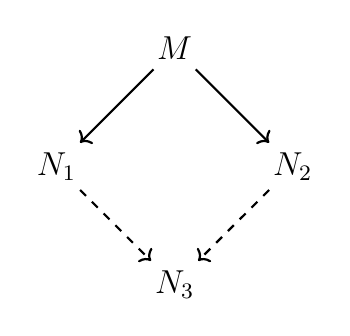
\begin{tikzpicture}[node distance=2.0cm, every node/.style={font=\large}]
  \node (t) at (0,0) {$M$};
  \node (t1) at (-1.5,-1.5) {$N_1$};
  \node (t2) at (1.5,-1.5) {$N_2$};
  \node (t3) at (0,-3) {$N_3$};
  \draw[->, thick] (t) -- (t1) node[midway, above left] {}; %{$\curly^*$};
  \draw[->, thick] (t) -- (t2) node[midway, above right] {}; %{$\curly^*$};
  \draw[->, dashed, thick] (t1) -- (t3) node[midway, below left] {}; %{$\curly^*$};
  \draw[->, dashed, thick] (t2) -- (t3) node[midway, below right] {}; %{$\curly^*$};
\end{tikzpicture}
\end{center}
The proof to this theorem is a quite lengthy, we would be miss the point
of this document if we were to introduce it [ChurchRosser].
\end{theorem}
\begin{corollary} Normalization: If a $\lambda$-term $M$ reduces to two normal forms $N_1$ and $N_2$, then they are alpha-equivalent:
\[
M \to_\beta^* N_1 \ \ \text{and} \ \ M \to_\beta^* N_2 \ \ \text{and $N_1$, $N_2$ are normal} \ \ \Rightarrow \ \ N_1 =_\alpha N_2
\]
\end{corollary}
The last and indeed the least important notion of equivalence:
\begin{definition} Two lambda terms \( M \) and \( N \) are said to be $\eta$-equivalent, written \( M =_\eta N \), if:
  \[
\begin{array}{@{}l@{\quad}l@{}}
  \inferrule*[right=\textsc{Eta}]
  { x \notin \FV M }
  { (\lam{x}{M}) =_\eta M   }
  &
  \inferrule*[right=\textsc{Abs}]
    { M =_\eta M' }
    { \lam{x}{M} =_\eta \lam{x}{M'} } \\[2ex]
  \inferrule*[right=\textsc{AppL}]
    { M_1 =_\eta M_1' }
    { M_1\,M_2 =_\eta M_1'\,M_2 }
  &
  \inferrule*[right=\textsc{AppR}]
    { M_2 =_\eta M_2' }
    { M_1\,M_2 =_\eta M_1\,M_2' }
\end{array}
\]

  The abstraction \( \lambda x.\, (M\;x) \) performs the same operation as \( M \), so if \( x \) is not used freely within \( M \), the abstraction is redundant.
\end{definition}
$\eta$-equivalence represents weak extensionality, since it does not encode observational equivalence. Two terms are observationally equivalent if they cannot be distinguished by any context that can be papplied to them.


\newpage
\subsection{\centering Some Important Constructions}

Within the \lcalc \ there exist a number of conventional constructions that represent key ideas in programming (numbers, booleans, branching and lists among others) In the following we define a few of the most important ones. These constructions can be used to prove relevant statements concerning the expressiveness of the \lcalc.

We begin defining $ \mathbb{N} $ for no particular reason. The notion of natural numbers in the \lcalc \ follows from the Peano axioms:
\begin{definition} Peano Axioms, the set of natural numbers $\mathbb{N}$
\begin{itemize}
\item (Zero) \( 0 \in \NAT \)
\item (Successor) \( \forall n \in \NAT, S(n) \in \NAT \)
\item (Initial) \( \forall n \in \NAT, S(n) \neq 0 \) \label{def:peano-nat-initial}
\item (Injectivity) \( \forall n, m \in \NAT, S(n) = S(m) \Rightarrow n = m \)
\item (Induction) \( P(0) \land \forall ( P(n) \Rightarrow P(S(n))) \Rightarrow \forall n,  P (n) \)
\end{itemize}
The first four axioms can be summarized using a graph:
\begin{center}
  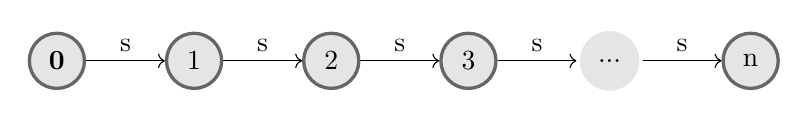
\begin{tikzpicture}[
    roundnode/.style={circle, draw=black!60, fill=gray!20, very thick, minimum size=7mm},
    emptynode/.style={circle, draw=black!0, fill=gray!20, very thick, minimum size=8mm}
    ]
    \node[roundnode]      (zero)                        {\textbf{0}};
    \node[roundnode]      (one)       [right=of zero]   {1};
    \node[roundnode]      (two)       [right=of one]    {2};
    \node[roundnode]      (three)     [right=of two]    {3};
    \node[emptynode]      (dots)      [right=of three]  {...};
    \node[roundnode]      (nth)       [right=of dots]   {n};

    \draw[->] (zero.east) -- node[midway, above] {s} (one.west);
    \draw[->] (one.east) -- node[midway, above] {s} (two.west);
    \draw[->] (two.east) -- node[midway, above] {s} (three.west);
    \draw[->] (three.east) -- node[midway, above] {s} (dots.west);
    \draw[->] (dots.east) -- node[midway, above] {s} (nth.west);
  \end{tikzpicture}
\end{center}
The last axiom is concerned with proving properties for all naturals given a precedent that satisfies the property and proof that if the property is satisfied for $n$ then it is satisfied for $n+1$, then the property is true of all naturals.
\end{definition}
\begin{example}
  Say for instance we mean to represent $ 3 $ using Peano notation, using the graph, we would come up with $ s(s(s(0))) $, since it is $3$ steps away from $0$.
\end{example}
\begin{definition} To add and multiply natural numbers one can just use following the sets of rules:
  \[
    n + m = 
    \begin{cases}
      n & \text{if } m = 0 \\
      s(n + m') & \text{if } m = s(m')
    \end{cases}
    \quad
    a \cdot b =
    \begin{cases}
      0 & \text{if } b = 0 \\
      a \cdot b' + a & \text{if } b = s(b')
    \end{cases}
  \]
\end{definition}
\begin{itemize}
\item \underline{$a + b$}: A recursive rule that performs the addition, and a base case to stop the recursion for n + 0, since there is no such number that has $ 0 $ as succesor.
\item \underline{$a \cdot b$}: Using addition we define multiplication in a similar way, adding $a$ as many times as the function $s$ is applied to $0$ in $b$.
\end{itemize}
\begin{definition} Representation of the set of all naturals in the realm of \lcalc, usually referred to as Church numerals:
  \label{def:church-naturals}
  \begin{align*}
    \texttt{0} &\equiv \la f.\la x. x \\
    \texttt{SUCC} &\equiv \la n. \la f. \la x . f ( n f x )
  \end{align*}
\end{definition}
\begin{example}
  The church numerals have been defined similarly to the peano axioms, that is, by bringing into existance an initial element and using the succesor function to define the rest of them. Let us apply \texttt{SUCC} a few times to illustrate:
  \begin{align*}
    \texttt{0} &\equiv \la f.\la x. x \\
    \texttt{1} &\equiv \la f.\la x. f x \\
    \texttt{2} &\equiv \la f.\la x. f f x \\
    \texttt{3} &\equiv \la f.\la x. f f f x \\
    \texttt{n} &\equiv \la f.\la x. f ^ n x
  \end{align*}
  where $ n $ denotes the number of times we append $ f $.
\end{example}
\begin{remark}
  Since \lterms \ are first-class citizens, and $f$ and $x$ are abstracted away, the reality is that numbers are a quite general construct that has many distinct applications. Recall Example \ref{ex:high-order-by-example} for instance.
\end{remark}
\begin{definition}
Now that we have a construction for the naturals, we can define some arithmetic operations:
\begin{align*}
  \texttt{ADD} &\equiv \la m.\la n. \la f. \la x. m f ( n f x) \\
  \texttt{MUL} &\equiv \la f.\la x. \la f. \la x. m (n f) x \\
  \texttt{ISZERO} &\equiv \lambda n. n\,(\lambda x.\texttt{FALSE})\,\texttt{TRUE}
\end{align*}
\end{definition}
\begin{example}
  \begin{center}
    \begin{align*}
      \texttt{ADD}\;\texttt{2}\;\texttt{3} &= (\la m.\la n.\la f.\la x. m\,f\,(n\,f\,x))\;(\la f.\la x. f\,f\,x)\;(\la f.\la x. f\,f\,f\,x) \\
                                           &\curly^* \la f.\la x.\; (\la f.\la x. f\,f\,x)\;f\;((\la f.\la x. f\,f\,f\,x)\;f\;x) \\
                                           &\curly^* \la f.\la x.\; (\la x. f\,f\,x)\;((\la x. f\,f\,f\,x)\;x) \\
                                           &\curly (\la f.\la x.\; f\,f\,f\,f\,f\,x) \\
                                           & \equiv \texttt{5} \quad \text{\magenta{Can I use alpha equiv o is it confusing?}}
    \end{align*}
  \end{center}
Multiplication works similarly to addition. As for \texttt{ISZERO}, the intuition behind it is that if the number is zero, then \(\lambda x.\, \texttt{FALSE}\) is dropped, and the result is \texttt{TRUE}; otherwise, it is applied at least once, which immediately yields \texttt{FALSE}.
\end{example}
\begin{remark}
  This proves that the \lcalc \ is capable of arithmetic, we leave them as a sidequest since we will not be extending or using them or in the rest of the text.
\end{remark}
The next constructions in line are the truth values of boolean logic, ``\textit{true}'' and ``\textit{false}'' for short.
\begin{definition} Boolean truth values:
  \begin{align*}
    \texttt{TRUE} &\equiv \lambda t.\lambda f. t \\
    \texttt{FALSE} &\equiv \lambda t.\lambda f. f
  \end{align*}
\end{definition}
\begin{remark}
  \label{rem:true-false}
  Note how $\TRUE \ M \ N \curly M $ and $ \FALSE \ M \ N \curly N $
\end{remark}
\begin{definition} Conditional, in other words \textit{``if statement''}.
  \begin{align*}
    \texttt{IF} &\equiv \lambda b.\lambda t.\lambda e. b\,t\,e
  \end{align*}
\end{definition}
The reality of the \IF \ is that it is just a combinator that happens to behave similarly to a branching statement whenever we pass a church encoded boolean as a first argument.
\begin{example} On the correct behabiour of $\IF$ i.e. check that it implements branching. $ M, N \in \La $ and $ \IF, \TRUE, \FALSE$ are as usual:
  \[
    \begin{aligned}
      & \IF \ \TRUE \ M \ N \\
      \equiv \ & (\la b.\la t.\la e.\, b\, t\, e) \ \TRUE \ M \ N  \\
      \curly \ & (\la t.\la e.\, \TRUE\ t\, e) \ M \ N  \\
      \curly \ & (\la e.\, \TRUE\ M\, e) \ N  \\
      \curly \ & \TRUE\ M\, N \curly^* M 
    \end{aligned}
    \quad
    \begin{aligned}
      & \IF \ \FALSE \ M \ N \\
      \curly^* \ & \FALSE\ M\, N \curly^* N
    \end{aligned}
  \]
  So the \IF \ just combines $b, t, e$ in such a way that whenever b is a church encoded boolean either $t$ or $e$ is dropped depending on the truth value of $b$. See Remark \ref{rem:true-false}. From this example we extract that $ \la x . x $ is equivalent to \IF \ it terms of behaviour, and thus, we could use $ \IF \equiv \la x . x $ interchangeably.
\end{example}
\begin{remark}
  Using the \IF \ we can implement an universal set of logic gates:
  \begin{align*}
    \NOT &\equiv \IF \, b \, \FALSE \, \TRUE \\
    \AND &\equiv \IF \, a \, (\IF \, b \, \TRUE \, \FALSE) \, \FALSE
  \end{align*}
  This allows us to simulate a nand gate, known to be universal \orange{\ref{} universality, conjunctive normal form}. Thus, the lambda calculus is at least equivalent to propositional logic \orange{\ref{} Something on turing completeness}.
\end{remark}
On the same track, another must-have for programmers is lists. Sice they are a bit more involved, we require tuples to define them. Note that the \IF \ is a tuple that contains two elements, we query the first element using a \TRUE \ i.e. the \textit{``then''} branch, and the sencond using a \FALSE \ i.e. the \textit{``else''} branch. We will be using this alternative definition for convenience:
\begin{definition} \( \PAIR \equiv \la x.\la y.\la f. f\,x\,y \)
\end{definition}
\begin{remark}
  This is more convenient since $ \PAIR \, M \, N \curly^* \la f . f \, M \, N  $, which allows us to query the first element using $ (\la f . f \, M \, N) \, \TRUE $ and the second by $ (\la f . f \, M \, N) \, \FALSE $, this motivates the definition below:
\end{remark}
\begin{definition}
\begin{align*}
  \FST &\equiv \la p. p\,(\la x.\la y. x) \\
  \SND &\equiv \la p. p\,(\la x.\la y. y)
\end{align*}
\end{definition}
\begin{proposition} A key property of $ \PAIR $'s is:
  \[\PAIR \, A \, B \equiv_\beta \PAIR \, (\FST \, A \, B) \, (\SND \, A \, B) \]
\end{proposition}
Using pairs, we now can define linear lists, we can achieve this using either left linear trees or right linear trees:
\begin{center}
  \[
    \begin{aligned}
      \begin{forest}
        [\rotatebox{60}{\texttt{\ldots}}
        [\PAIR
        [\PAIR
        [\NIL]
        [\texttt{ELEM}]
        ]
        [\texttt{ELEM}]
        ]
        [\texttt{ELEM}]
        ]
      \end{forest}
    \end{aligned}
    \hspace{1cm}
    \textit{or}
    \hspace{1cm}
    \begin{aligned}
      \begin{forest}
        [\rotatebox{-60}{\texttt{\ldots}}
        [\texttt{ELEM}]
        [\PAIR
        [\texttt{ELEM}]
        [\PAIR
        [\texttt{ELEM}]
        [\NIL]
        ]]]
      \end{forest}
    \end{aligned}
  \]
\end{center}
\begin{definition} We define \NIL \ in the same way we defined \texttt{0} and \FALSE \ before: $ \NIL \equiv \la f.\la z. z $; \NIL \ represents the terminating element of the inductive definition for lists. To build lists, we cons lists together using:
  \[ \texttt{CONS} \equiv \la h.\la t.\la f.\la z. f\,h\,(t\,f\,z) \]
that binds a new element $h$ to to an pre-existing list or to \NIL.
\end{definition}
\begin{note}
  This notion of inductively defined lists is lays the foundations of the \textbf{LISP} family of programming languages, hence the name (LISt Processing).
\end{note}
\begin{definition} Relevant list operators:
\begin{align*}
  \texttt{ISNIL} &\equiv \la l. l\,(\la h.\la t. \FALSE)\,\TRUE \\
  \texttt{HEAD} &\equiv \la l. l\,(\la h.\la t. h)\,\text{undef}
\end{align*}  
\end{definition}


\newpage
\magenta{Turing completeness of the \lcalc}
\begin{align*}
  \texttt{CONS} &\equiv \la h.\la t.\la f.\la z. f\,h\,(t\,f\,z) \\
  \texttt{IS\_NIL} &\equiv \la l. l\,(\la h.\la t. \texttt{FALSE})\,\texttt{TRUE} \\
  \texttt{HEAD} &\equiv \la l. l\,(\la h.\la t. h)\,\text{undef} \\
  \texttt{TAIL} &\equiv \la l.\, \texttt{FIRST}\,(l\,(\la p.\la h.\, \texttt{PAIR}\,(\texttt{SECOND}\,p)\,(\texttt{CONS}\,h\,(\texttt{SECOND}\,p)))\,(\texttt{PAIR}\,\texttt{NIL}\,\texttt{NIL}))
\end{align*}
\textbf{Recursion:}
\begin{align*}
  \texttt{Y} &\equiv \lambda f.(\lambda x. f\,(x\,x))\,(\lambda x. f\,(x\,x))
\end{align*}


\newpage
\subsection{\centering Fixed Point Combinators and Recursion}
\label{sec:recursion-fixed-points}
\magenta{Reintroduce the question from before}
From the Church Rosser Property of confluence, we know that whenever a term has a normal form, this normal form must be unique. We still have not given an answer to whether all \lterms \ have a normal form.

The most straight forward way to test this, is to check whether there exists some term that reduces to itself, effectively creating a loop in the $\beta$-reduction chain so to speak. In more formal terms this means there exists some $M$ such that \( M \curly^n M \) with $ n > 0 $. It turns out \( \Omega \equiv (\la x . \, x \, x) (\la x . \, x \, x) \) fullfills this requirement. Let us inspect what goes on while $\beta$-reducing this term:
\[
  \Omega \equiv (\la x . \, x \, x) (\la x . \, x \, x) \curly (\la x . \, x \, x) (\la x . \, x \, x) \curly^* (\la x . \, x \, x) (\la x . \, x \, x) \equiv \Omega
\]
This so called $\Omega$-combinator, proves that not all terms have a normal form, and shines a beam of light onto how recursion can be achieved in the \lcalc.

There is one caveat to this, that classically, recursion is achieved through naming, take for instance this definition for the $\mathrm{gdc}$:
\begin{align*}
  \underline{\mathrm{gcd}}(a,b) &= 
                      \begin{cases}
                        a & b = 0 \\
                        \underline{\mathrm{gcd}}(b,\, a \bmod b) & b \neq 0
                      \end{cases}
\end{align*}
Here, when $b \neq 0$ the name gcd is used to refer to the same definition again. In the \lcalc \ such self-referencing definitions are not permited since the language does not allow names. To bypass this setback the notion of fixed point is of particular interest.
\begin{definition}
  Let \( f : X \to X \) be a function. An element \( x \in X \) is called a fixed point of \( f \) if \( f(x) = x. \)
\end{definition}
\begin{example} Some simple functions that illustrate what fixed points are:
  \[
    \begin{tabular}{|c|c|}
      \hline
      \textit{Function} & \textit{Fixed Point(s)} \\
      \hline
      $f(x) = c$ & $x = c$ \\
      \hline
      $g(x) = x$ & $\{ x \mid x \in \mathbb{R} \}$ \\
      \hline
      $h(x) = x^2$ & $ x = 0,\, x = 1 $ \\
      \hline
    \end{tabular}
  \]
\end{example}
This harmless idea satisfies an interesting property, namely that $ x = f(x) = f(f(x)) = f^n(x) $ effectively creating a chain every element $ f^{n+1}(x) = f(f^{n}(x))$, thus attaining self-reference without naming. This idempotent behaviour under application is important, since it showcases the ability of fixed points to induce recursion. Our quest now, is to find a term that simulates this behaviour. To do this, let us translate the definition for fixed point into the $\lambda$-world.
\magenta{maybe use circ (i.e function composition) in the chain since it might have some meaning in the context of categories}.
\begin{definition}
  Given a lambda term \( L \in \La \), a term \( M \in \La \) is called a fixed point of \( L \) if \( M =_\beta L M \).
\end{definition}
No surprises here, the definition is close to a one-to-one mapping of its functional counterpart seen previously. Interestingly enough, it turns out that every lambda term has a fixed point, as stated in the theorem proven below:
\begin{theorem}
  For every \( L \in \La \), there exists \( M \in \La \) such that $ M $ is a fixed point for $ M $ i.e. $ M =_\beta L M $. Referred to as the Fixed Point Theorem in the literature.
\end{theorem}
\begin{proof} Given $L \in \La$, define $M$ as below:
  \[
    M := (\la x . \, L \, (x \, x))(\la x . \, L \, (x \, x))
  \]
  $M$ is a reducible expression, redex for short:
  \begin{align*}
    M 
    &\equiv (\la x . \, L \, (x \, x))(\la x . \, L \, (x \, x)) \\
    &\curly L \, ((\la x . \, L \, (x \, x))(\la x . \, L\, (x \, x))) \\
    &\equiv L \, M.
  \end{align*}
  Hence, $ M =_\beta L M $, as required.
\end{proof}
\begin{remark}
  See how $ L M $ is the application of $ M $ to $ L $ and that using \textsc{AppR} we can keep $\beta$-reducing $ M $ the same way we did for $ x = f(x) = f(f(x))\dots $ only this time using lambda terms:
  \[
    M \curly L \, M \curly L \, L \, M \curly^* L^n M.
  \]
\end{remark}
Now that nameless self-reference has been proven to exist within the the \lcalc, we take a step forward and introduce a few of the most important fixed point combinators and explore their different natures.
\begin{definition} $Y$ Combinator. \orange{The term that given some other term returns its fixed point.}
\[
  Y \triangleq \la f.\, (\la x.\, f\, (x\, x))\, (\la x.\, f\, (x\, x))
\]
\end{definition}
\begin{note}
  \( Y \equiv \la L . M  \) \magenta{M defined previously. Improve this, find some other way to put it? note it is an improved $\Omega$}
\end{note}
\begin{remark}
  Even though the $Y$ combinator is of theoretical interest since it allows us to find recursion within the \lcalc, it is of little practical use since it always runs into non-termination e.g.
  \[
    \begin{aligned}
      Y \, F &\equiv (\la f. \, (\la x . \, f \, (x \, x))(\la x . \, f \, (x \, x))) F \\
      &\curly (\la x . \, F \, (x \, x))(\la x . \, F \, (x \, x)) \\
             &\curly F((\la x . \, F \, (x \, x))(\la x . \, F \, (x \, x))) \\
             &\curly F(F((\la x . \, F \, (x \, x))(\la x . \, F \, (x \, x)))) \\
             &\curly \cdots
    \end{aligned}
  \]
  This is due to its lazy nature, this means that the argument $F$ is not evaluated until $Y$ is done unravelling i.e. never.
\end{remark}
To work arround this issue, several other combinators exist, one of the most notorious, the $Z$ combinator is defined next:
\begin{definition} $Z$ combinator
\[
  Z \triangleq \la f.\, (\la x.\, f\, (\la v.\, x\, x\, v))\, (\la x.\, f\, (\la v.\, x\, x\, v))
\]
\end{definition}
\begin{example}
  \[
    \begin{aligned}
      Z \, F &\equiv (\la f.\, (\la x.\, f\, (\la v.\, x\, x\, v))\, (\la x.\, f\, (\la v.\, x\, x\, v)))\, F \\
             &\curly (\la x.\, F\, (\la v.\, x\, x\, v))\, (\la x.\, F\, (\la v.\, x\, x\, v)) \\
             &\curly F\, (\la v.\, (\la x.\, F\, (\la v.\, x\, x\, v))\, (\la x.\, F\, (\la v.\, x\, x\, v))\, v)\, \\
             &\equiv F\, (\la v.\, Z \, F \, v)\, \\
    \end{aligned}
  \]
\end{example}


\newpage

\section{\centering Simply Typed \lCalc}

We covered the untyped \(\lambda\)-calculus, highlighting its strengths and limitations. This  
section introduces the notion of typing, which restricts its expressiveness while  
improving the tractability of studying its properties. The idea of typing arises  
from the usual definition of a function, understood as a mapping between elements of sets. For example, consider a function  
\( f : A \to B \) defined by \( a \mapsto f(a) \), to develop the analogy.

Notice how we are able to recognize \(A\) as the domain and \(B\) as the codomain, and how the mapping  
is meaningful only within this context—otherwise \( f \) would lack sense and  
purpose. Hence, it is important to first restrict the environment in which \( f \)  
lives and then remain within it while defining the mapping. In this instance,  
that means using constructions and operations that exist within the realms of  
\(A\) and \(B\).

In the context of the \(\lambda\)-calculus, types serve as a means of restriction, similar  
to how we use logical predicates to define sets. Just as \( f : \mathbf{?} \to \mathbf{?} \) is refined  
to \( f : A \to B \) by specifying requirements on the arguments and ensuring  
properties of the outputs, we use types to impose requirements on the arguments  
of an abstraction and to ensure properties of the reduction process of that term.

Since the \(\lambda\)-calculus treats all terms as first-class citizens, attempting to impose  
restrictions directly on arguments is not effective. Instead, we define restrictions  
on all terms by pairing each term with additional information called a \emph{type}.  
This tells us about the nature of a given term, which may be of two kinds: a simple  
type or a function type (written as \(\to\)). Because \(\Lambda\) is infinite, we require  
a set of rules that automatically assigns types to terms.

Introducing a typing system into the \(\lambda\)-calculus splits \(\Lambda\) into two categories:  
Typable and Non-typable terms. These sets are disjoint, and the separation is strict  
and exhaustive. This simple type system classifies expressions such as  
\( x (\lambda y.y) \) or \( Y \) as untypable, while expressions such as \( \lambda x.x \) have type  
\(\alpha \to \alpha\).

Let us now proceed by introducing some of the necessary concepts required to type \(\lambda\)-terms.

\begin{definition} The set of all types, $\Ty$:
  
  Let $\Tb = \{ \alpha, \beta, \gamma, \dots \}$ be the set of all basic type, usually denoted using symbols from the greek alphabet.
  
  ...
  
  \begin{align*}
    \texttt{<type>} &\;\texttt{::=}\; \texttt{<atom>} \\
                    &\;\texttt{|}\; \texttt{"("}\ \texttt{<type>}\ \texttt{"$\to$"}\ \texttt{<type>}\ \texttt{")"} \\
    \texttt{<atom>} &\;\texttt{::}\in \Tb
  \end{align*}
\end{definition}



%\orange{
%The Untyped Lambda Calculus in computationally equivalent to a  Turing machine. However, with great computational power comes limited decidability of properties, leading to non-termination, or expressions such as $x(\lambda y . y)$, whose meaning is unclear.
%A classic example of non-termination is the $Y$ combinator, however, the Simply Typed Lambda Calculus does not allow such expressions, as its type system is unable to assign a valid type to them.
%\magenta{if there is a proof of turing completeness, add how if we remove combinators then we remove turing completeness i.e. finite tape $\neq$ turing complete}
%To understand why, consider the role of function types: in the world of functions, a function maps values from a domain to a range. The Simply Typed Lambda Calculus enforces this structure explicitly, ensuring that every function application is well-typed and preventing self-application patterns that would lead to paradoxes or infinite loops.
%Having grasped the untyped lambda calculus's Turing completeness and ability to compute all computable functions, we now seek properties related to decidability. To this end, we introduce the simply typed lambda calculus. Although it possesses less computational power than its untyped counterpart, it offers attractive features regarding decidability that will be useful later on.
%}

\orange{typing a la church, typing a la curry}














\chapter{Category Theory}
\orange{Category Theory...}


\begin{definition}
A \emph{category} \( \cat{C} \) consists of:
\begin{itemize}[nosep]
  \item A class \( \Ob(\cat{C}) \) of \emph{objects},
  \item For each pair \( A, B \in \Ob(\cat{C}) \), a set \( \Hom_{\cat{C}}(A, B) \) of \emph{morphisms} (also called \emph{arrows}) from \( A \) to \( B \),
\end{itemize}
such that composition of morphisms and identity morphisms are defined and satisfy associativity and unit laws.
\end{definition}



\end{document}

